% 03_results.tex
\providecommand{\todo}[1]{\textbf{[TODO: #1]}}

\section{Results}
\noindent
This section reports the three experiments described in the Methods section: computational cost, aliasing, and filter stability. Each is shown with one figure. All measurements use a sample rate of 48\,kHz and a block size of 128 samples, so one block must be processed in at most 2.67\,ms (2666.67\,$\mu$s) to keep up with real time.

%----------------------------------------------------------------------
\subsection{Computational Overhead: Oscillators}
\label{sec:res_cpu_osc}
\noindent
Table~\ref{tab:cpu_osc} compares the mean processing time per 128-sample block for the naive and band-limited (PolyBLEP for the sawtooth and square, PolyBLAMP for the triangle) oscillator cores. The pitch used was a B6---the highest pitch possible in picoDAW---the filter was bypassed, and the trace length is about 30\,s, i.e., 11{,}250 blocks. 

The complete \texttt{AudioWorkletProcessor::Process} duration, which includes both the DSP calculations and the relevant browser overhead, is used as the key metric, to provide a more realistic view of the overall effect of different algorithms on computational efficiency.

\begin{table}[htbp]
  \centering
  \caption{Mean processing time per block ($\mu$s) for naive and band-limited oscillators.}
  \label{tab:cpu_osc}
  \begin{tabular}{lrrrr}
    \hline
    Waveform & Naive & Band-limited & Difference & Relative \\
    \hline
    Sawtooth (PolyBLEP)  & 54.59 & 53.54 & $-1.05$ & $-1.9\%$ \\
    Square (PolyBLEP)    & 56.38 & 56.98 & $+0.60$ & $+1.1\%$ \\
    Triangle (PolyBLAMP) & 57.01 & 58.95 & $+1.94$ & $+3.4\%$ \\
    \hline
  \end{tabular}
\end{table}

The band-limited oscillators cost almost the same as the naive ones. The largest difference is for the triangle, where PolyBLAMP adds 1.94\,$\mu$s per block (3.4\%). For the square wave the increase is 0.60\,$\mu$s (1.1\%), and for the sawtooth the band-limited core was measured as slightly \emph{faster} than the naive one (by 1.05\,$\mu$s). All six configurations lie between 53.5 and 59.0\,$\mu$s, so the highest cost (the PolyBLAMP triangle) uses 2.21\% of the 2666.67\,$\mu$s block budget.

The sawtooth result should not be taken to mean that PolyBLEP is genuinely cheaper than a naive sawtooth. An algorithm that adds correction terms cannot do less work than the one it extends, and the difference of about 1\,$\mu$s is comparable to the run-to-run variation seen between measurements elsewhere in this section; like in the following comparison between filters. Each value is a single trace, so the safe reading is that the band-limited cores cost about the same as the naive ones, within a few microseconds, and that the triangle is the most expensive of the three.

\subsection{Computational Overhead: Filters}
\label{sec:res_cpu}
\noindent
Figure~\ref{fig:cpu} and Table~\ref{tab:cpu} show the mean processing time per 128-sample block for the Biquad IIR and ZDF SVF filters as the LFO modulating the cutoff is swept from 0 to 50\,Hz.

\begin{figure}[htbp]
  \centering
  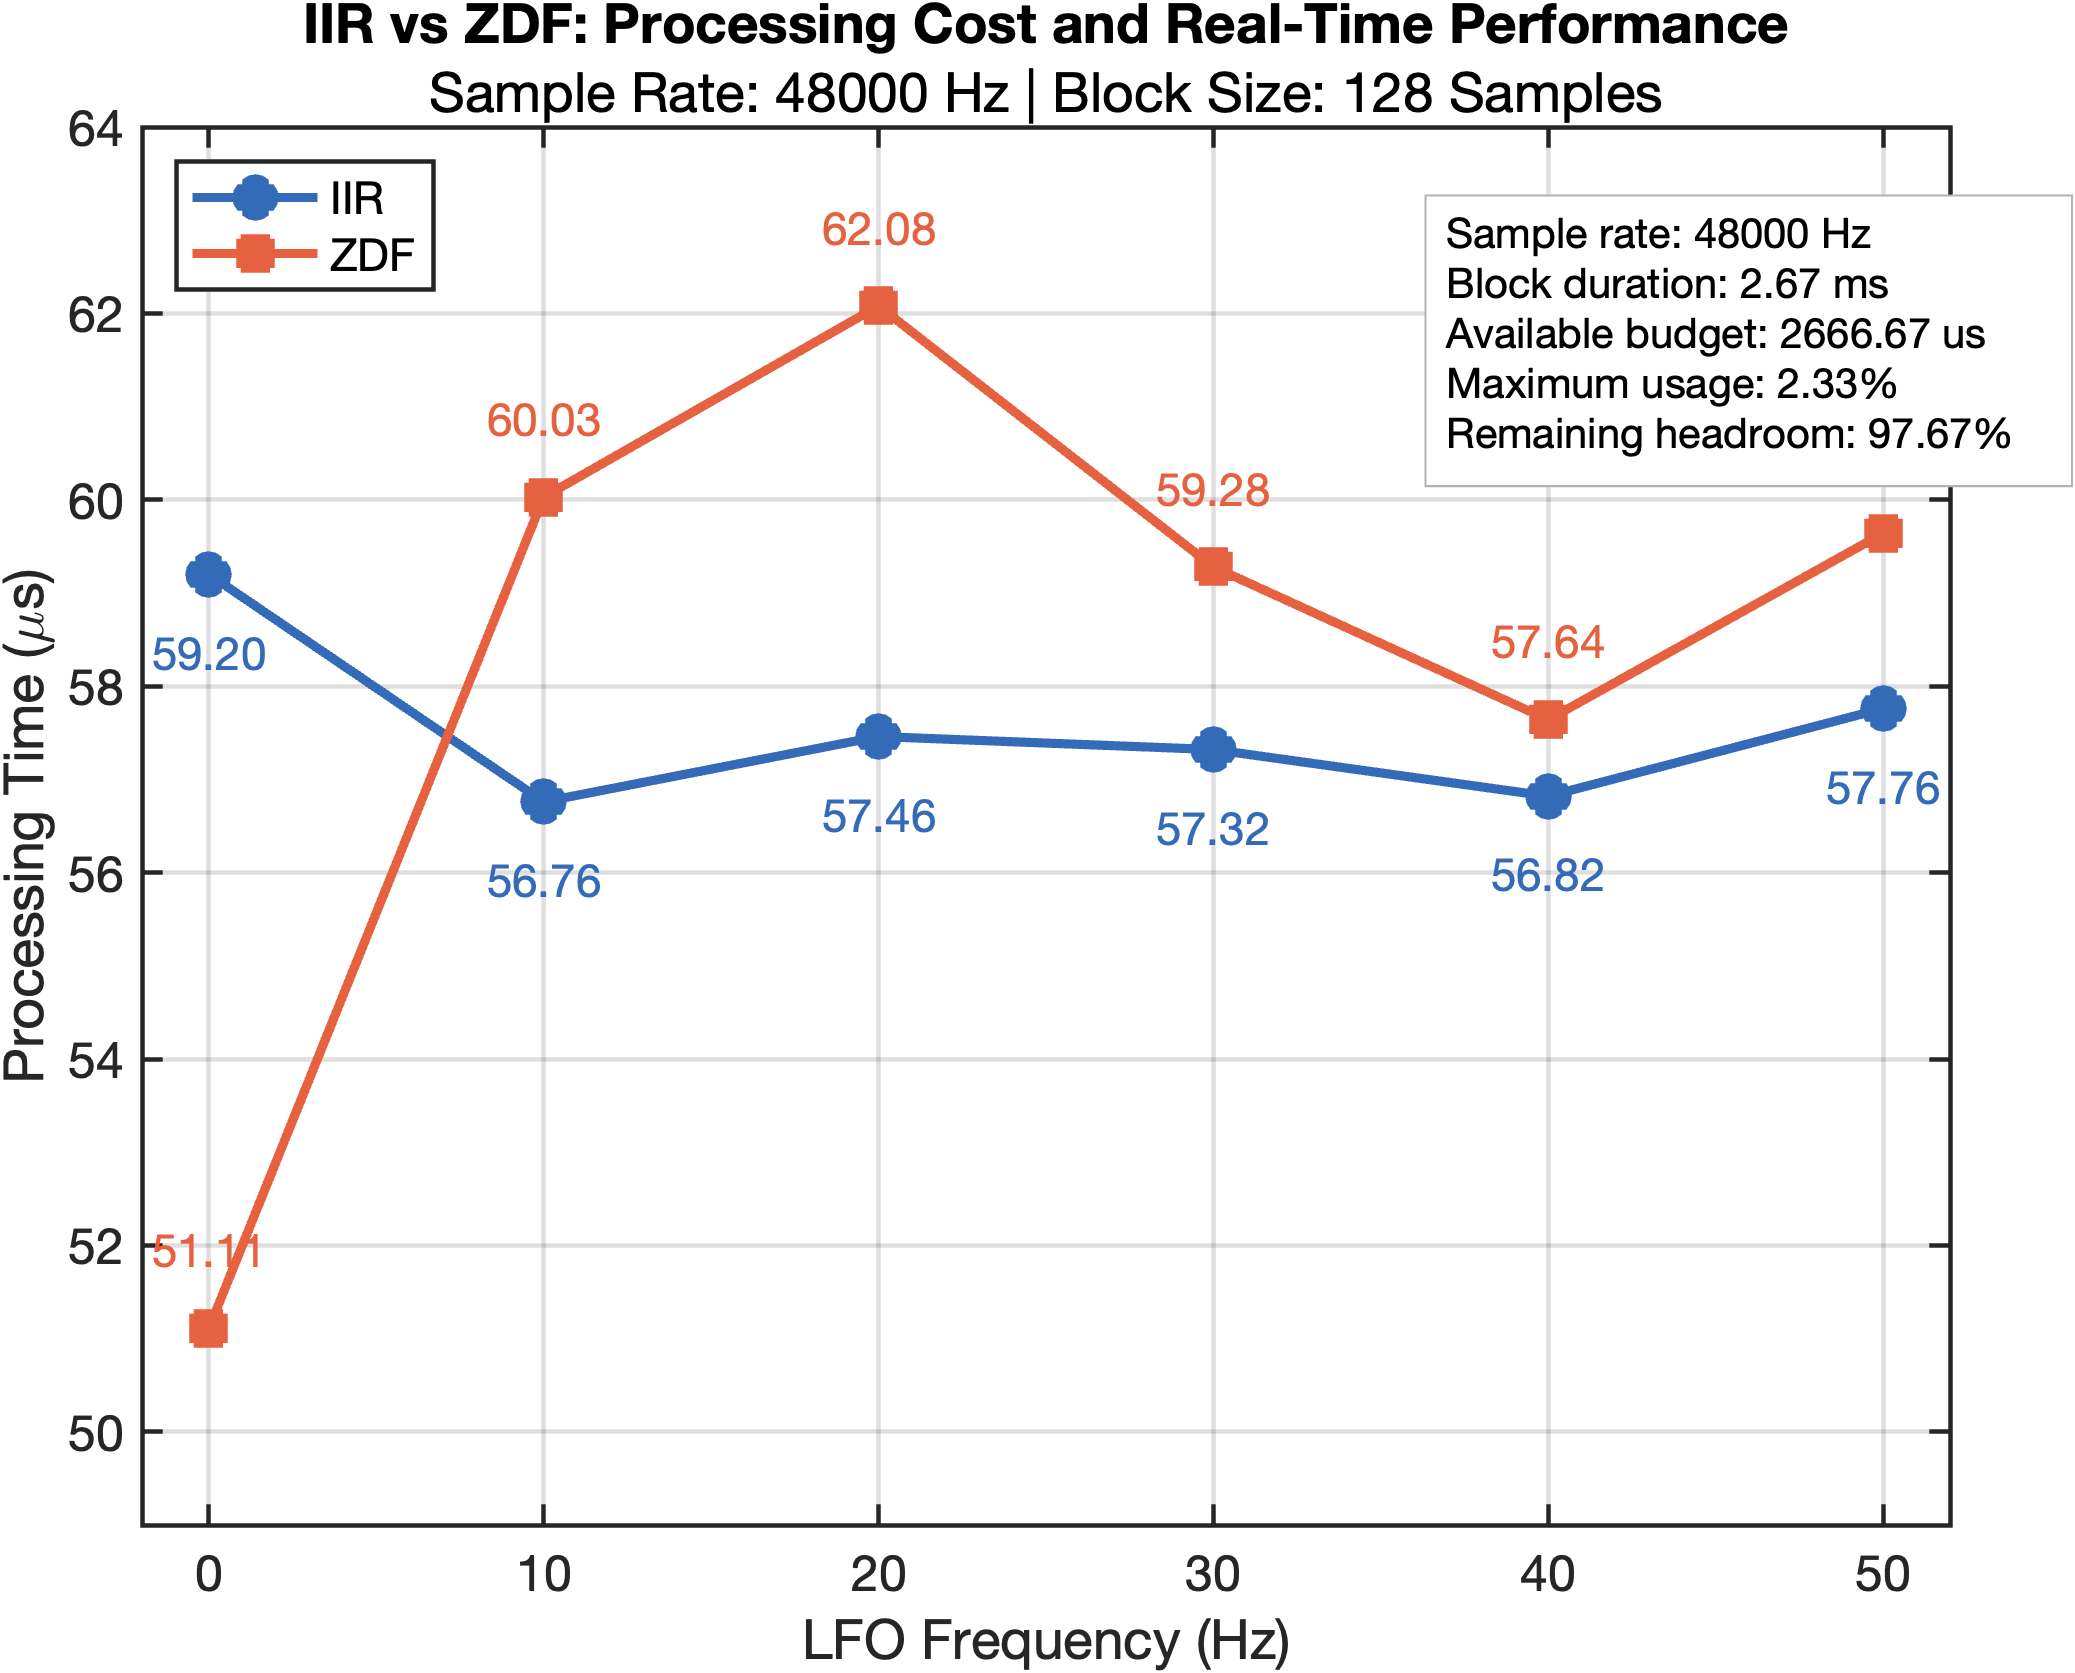
\includegraphics[width=0.85\linewidth]{figures/exp1_cpu.png}
  \caption{Mean processing time per 128-sample block for the Biquad IIR and ZDF SVF filters versus LFO frequency (48\,kHz sample rate). The maximum recorded cost corresponds to 2.33\% of the block budget.}
  \label{fig:cpu}
\end{figure}

\begin{table}[htbp]
  \centering
  \caption{Processing time per block ($\mu$s) for each filter, and the delta difference}
  \label{tab:cpu}
  \begin{tabular}{rrrr}
    \hline
    LFO (Hz) & IIR & ZDF & $\text{ZDF}-\text{IIR}$ \\
    \hline
    0  & 59.20 & 51.11 & $-8.09$ \\
    10 & 56.76 & 60.03 & $+3.27$ \\
    20 & 57.46 & 62.08 & $+4.62$ \\
    30 & 57.32 & 59.28 & $+1.96$ \\
    40 & 56.82 & 57.64 & $+0.82$ \\
    50 & 57.76 & 59.64 & $+1.88$ \\
    \hline
  \end{tabular}
\end{table}

Both filters are very cheap relative to the real-time budget. Every measurement lies between roughly 51 and 62\,$\mu$s, and the highest value (ZDF at 20\,Hz, 62.08\,$\mu$s) uses 2.33\% of the block budget, leaving 97.67\% headroom.

For LFO frequencies from 10 to 50\,Hz the ZDF filter is consistently the more expensive of the two, by between about 1 and 5\,$\mu$s per block (an average of roughly 2.5\,$\mu$s, or about 4\%). The IIR cost is almost flat across LFO frequency (56.8 to 57.8\,$\mu$s in this range), whereas the ZDF cost varies more, with no monotonic trend.

The 0\,Hz point does not follow this pattern: ZDF is cheaper than IIR (51.11 against 59.20\,$\mu$s). Each point comes from a single trace without repetition, so differences of a few microseconds should be read cautiously, and this point may again reflect run-to-run variation rather than a real effect. This is returned to in the discussion.

%----------------------------------------------------------------------
\subsection{Aliasing}
\label{sec:res_alias}
\noindent
Figure~\ref{fig:alias} compares the spectra of the naive and PolyBLEP sawtooth cores at a fundamental of 1760\,Hz (top), and the aliasing energy $E_{\text{alias}}$ defined in the methods section; see equation (14).

\begin{figure}[htbp]
  \centering
  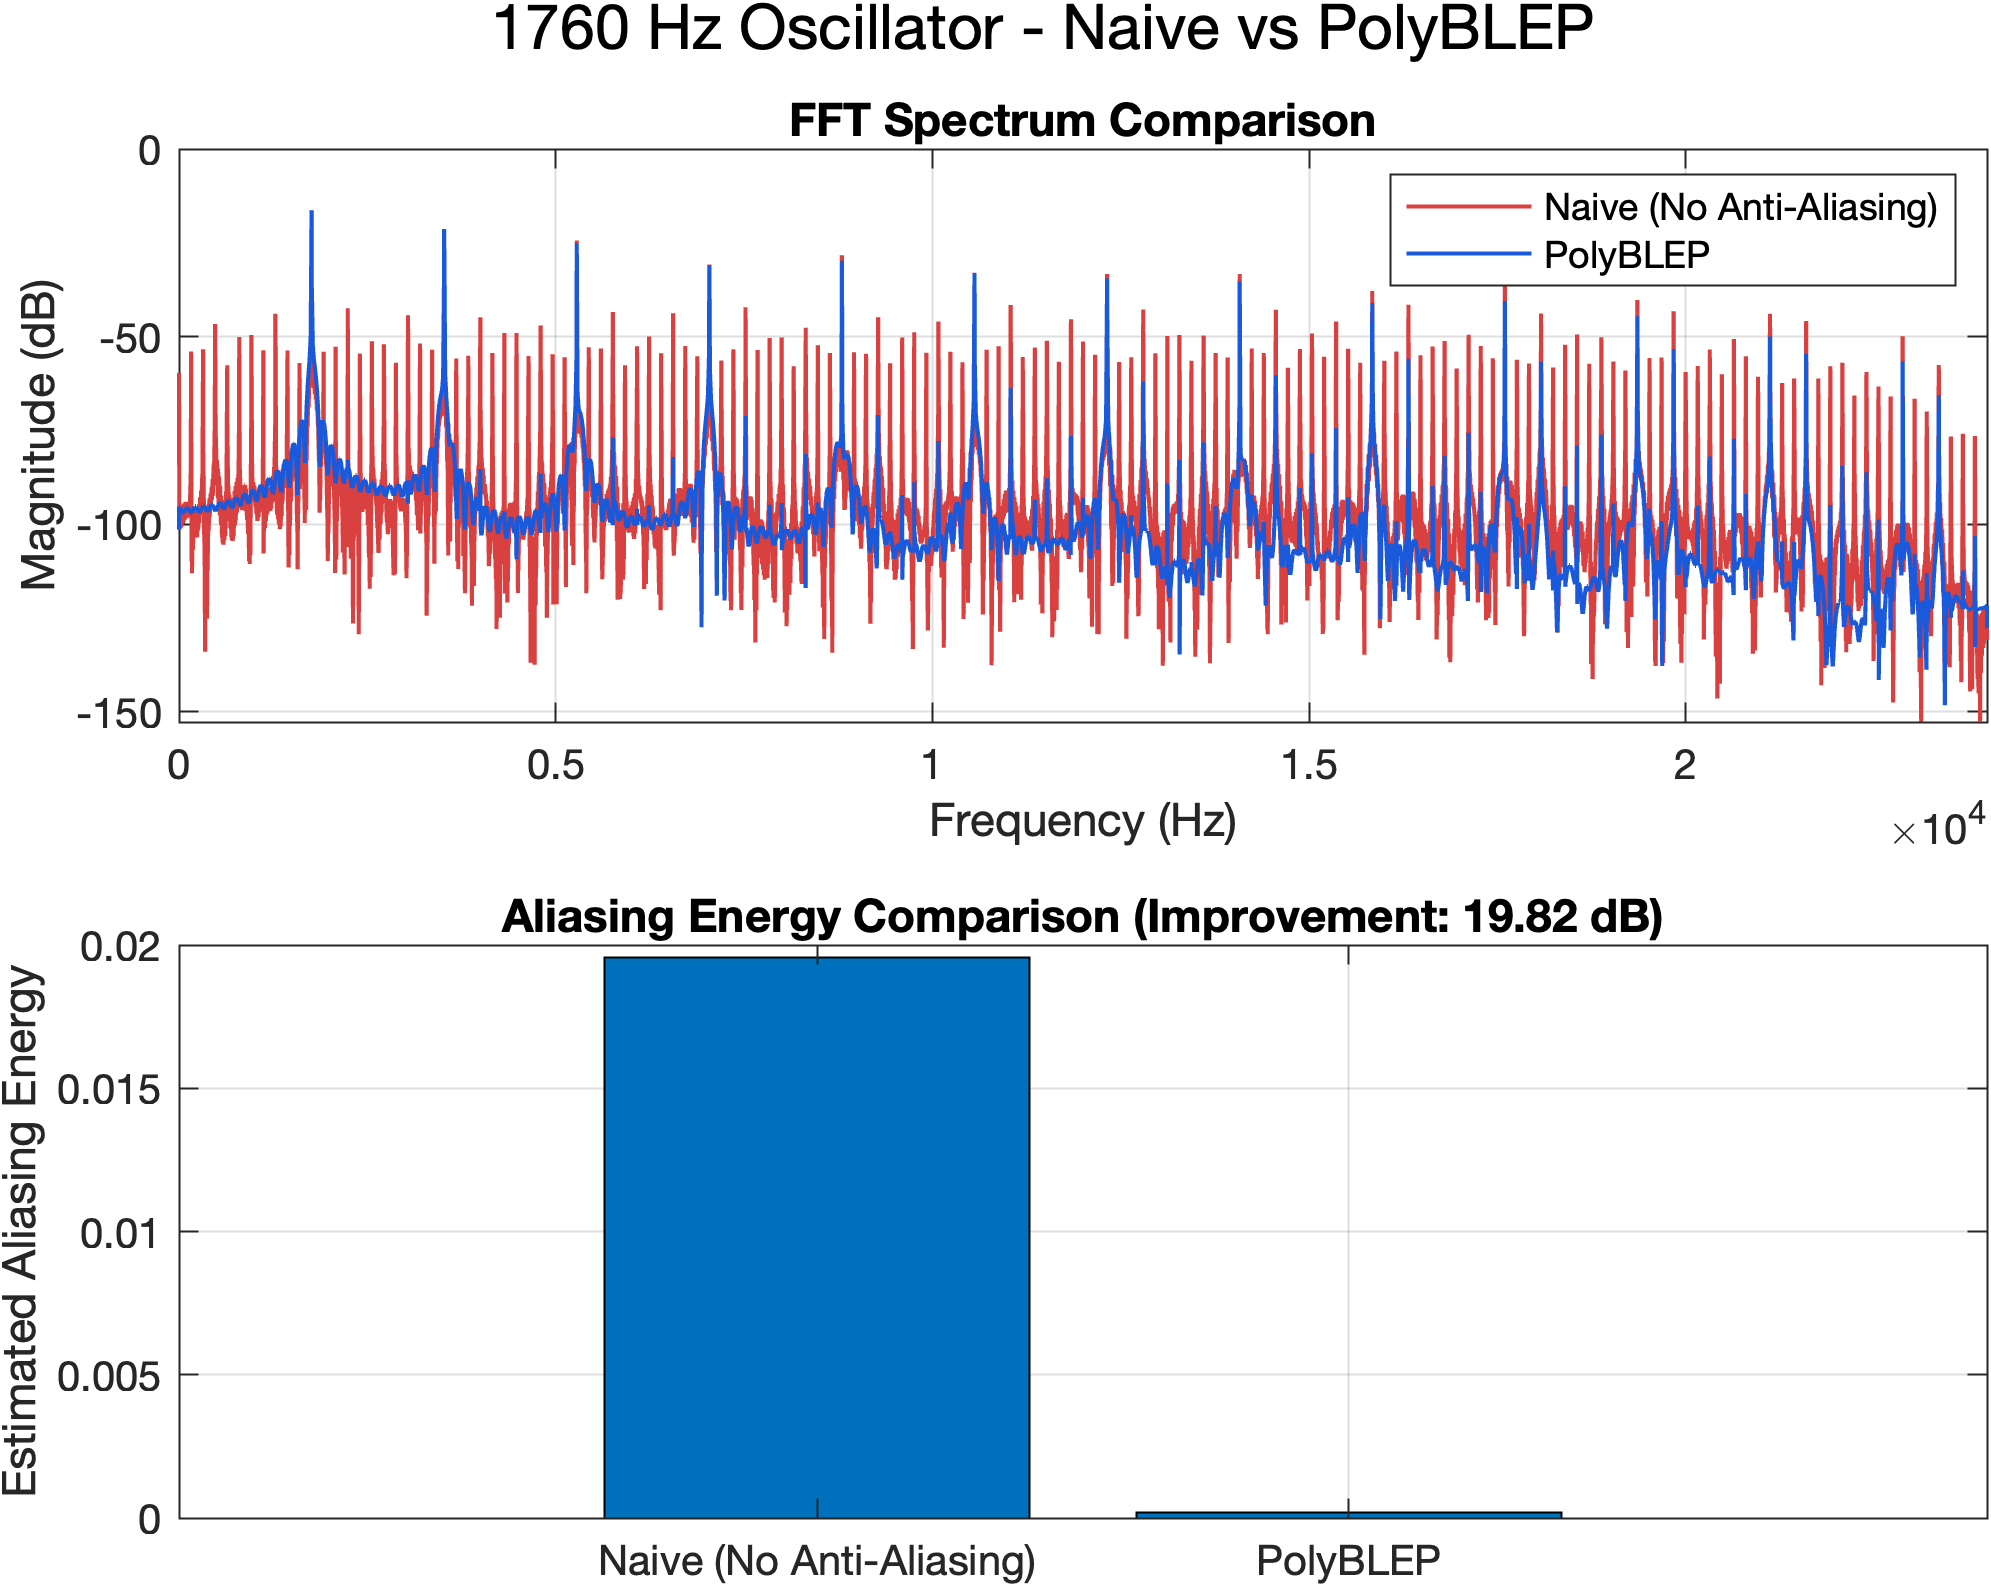
\includegraphics[width=\linewidth]{figures/exp2_alias.png}
  \caption{Top: magnitude spectra of a 1760\,Hz sawtooth from the naive and PolyBLEP cores. Bottom: estimated aliasing energy for each core. The improvement is 19.82\,dB.}
  \label{fig:alias}
\end{figure}

In the spectrum, both cores show the same harmonic peaks at multiples of 1760\,Hz. However, the two differ in everything between the harmonics. The naive core shows a dense comb of inharmonic lines across the whole band. These include lines below the fundamental, where an ideal sawtooth has no energy. 

These are the harmonics above Nyquist folded back into the audible range; the aliasing. With PolyBLEP, the same lines are mostly absent and the spectrum between harmonics falls to a noise floor of about $-90$ to $-100$\,dB, an improvement of tens of decibels. Some small residual lines remain around the harmonics, and the upper harmonics of the PolyBLEP signal appear slightly lower than those of the naive signal. The aliasing-energy measure agrees with this. PolyBLEP reduces $E_{\text{alias}}$ by 19.82\,dB, a factor of about 96 in energy.

%----------------------------------------------------------------------
\subsection{Filter Stability}
\label{sec:res_stability}
\noindent
Figure~\ref{fig:stability} shows the output of the ZDF and Biquad IIR filters under the same extreme modulation: an LFO rate of 150\,Hz, a base cutoff of 57\,Hz, and resonance set to 100\%.

\begin{figure}[htbp]
  \centering
  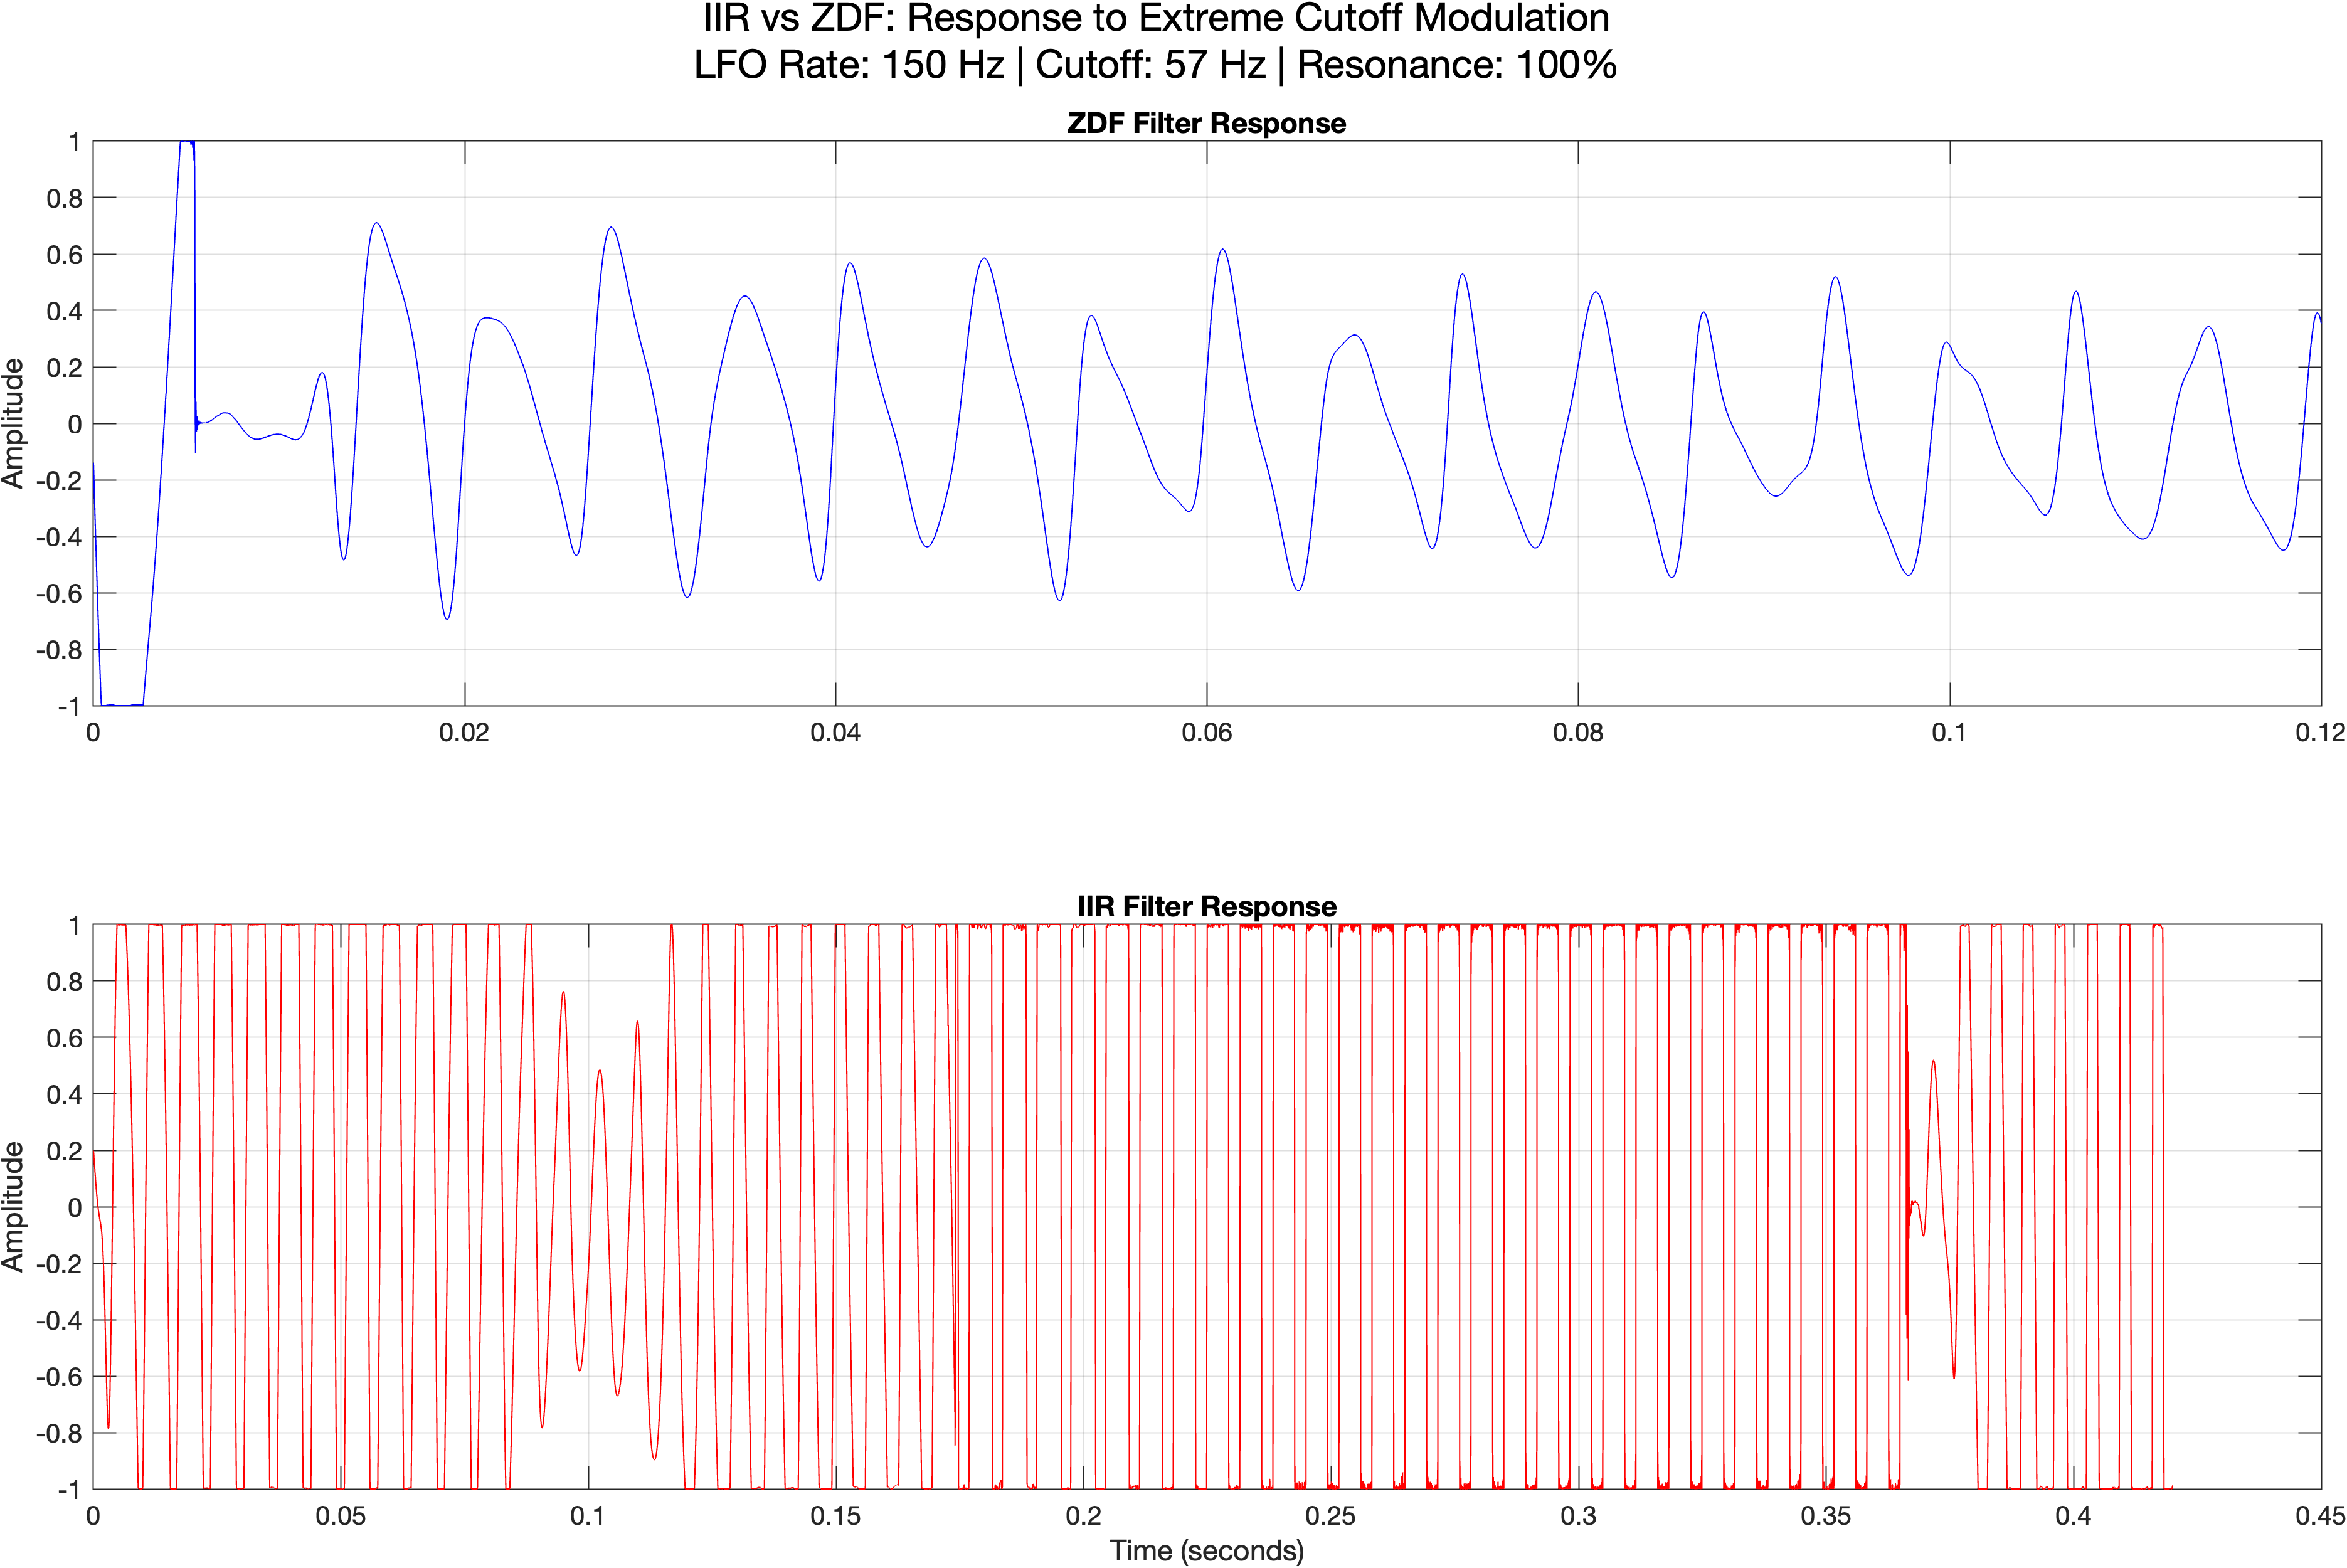
\includegraphics[width=\linewidth]{figures/exp3_stability.png}
  \caption{Filter output under extreme cutoff modulation (LFO 150\,Hz, cutoff 57\,Hz, resonance 100\%). Top: ZDF SVF. Bottom: Biquad IIR.}
  \label{fig:stability}
\end{figure}

The two filters behave very differently. The ZDF output shows a brief onset transient, reaching full scale ($\pm 1$) for a few milliseconds at the start. It then settles into a bounded, modulated oscillation with peaks of roughly 0.4 to 0.7 and no further saturation over the plotted window.

The IIR output instead repeatedly swings between the limits of $-1$ and $+1$ and spends most of the plotted time clipped there, giving a square-like waveform. There are short stretches (around 0.09 to 0.12\,s and again near 0.37\,s) where the amplitude drops below full scale, but it returns to saturation each time. This is the behaviour of a feedback instability, not of a well-behaved filter with a loud signal. In listening, the IIR case produced extremely loud, harsh output, whereas the ZDF case did not.

However, since the output is limited to $[-1,1]$, the plot shows only that the IIR output saturated, not how far its internal state had grown, a limitation of the experimental method. The effect of ZDF in stabilising the filter output was certainly noticable though; the ZDF switch was even used during this experiment as a panic button to turn off the tremendously loud signal from the IIR filter when pushed to the extreme.

%----------------------------------------------------------------------
\subsection{Summary of Results}

Taken together, the results give the following picture. Anti-aliasing with PolyBLEP reduced aliasing energy by almost 20\,dB at 1760\,Hz. The ZDF filter cost a few microseconds more per block than the Biquad IIR, but remained stable under modulation that drove the IIR into sustained saturation. All the filter configurations tested used no more than 2.33\% of the real-time budget.